\documentclass{beamer}

\usepackage[utf8]{inputenc}
\usepackage{graphicx} 


%Information to be included in the title page:
\title{Laboratorio 2}
\author{Alvaro Frias Garay - Ary Lautaro Di Bartolo}
\institute{Universidad Nacional de Córdoba - Universidad Nacional de Cuyo}
\date{2021}



\begin{document}

\frame{\titlepage}


\begin{frame}
    \frametitle{Autovectorización}
    gcc -O1 -ftree-vectorize -fopt-info-vec 
    -fopt-info-vec-missed wtime.c mtwister.c tiny\_mc.c -lm

\end{frame}

\begin{frame}
    \frametitle{Autovectorización}
    \begin{itemize}
        \item<1-> tiny\_mc.c:107:5: missed: couldn't vectorize loop
        \item<2-> tiny\_mc.c:107:5: missed: not vectorized: multiple nested loops.
        \\\pause

        \item <3-> tiny\_mc.c:78:16: missed: couldn't vectorize loop
        \item <4-> tiny\_mc.c:78:16: missed: not vectorized: control flow in loop.
        \\\pause
        \item <5->tiny\_mc.c:71:9: missed: couldn't vectorize loop
        \item <6->tiny\_mc.c:71:9: missed: not vectorized: number of iterations cannot be computed.
        \\\pause
    \end{itemize}
\end{frame}

\begin{frame}
    \frametitle{Autovectorización}

    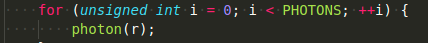
\includegraphics[width=4in]{imagenes/autovector_f1.png} \pause
    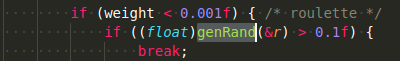
\includegraphics[width=4in]{imagenes/autovector_f2.png} \pause
    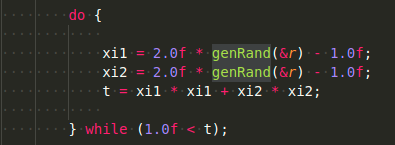
\includegraphics[width=4in]{imagenes/autovector_f3.png} 

\end{frame}

\begin{frame}
    
\includegraphics[width=4cm]{imagenes/spongebobmeme.jpg} 
    Vectorización Manual
\end{frame}

\begin{frame}
    \frametitle{Vectorización Manual}
    \begin{itemize}
        \item Intel Intrisinsics \pause
        \item AVX / AVX-2 \pause
        \item Vectores de 256 bits i.e 8 floats
    \end{itemize}
\end{frame}

\begin{frame}
    \frametitle{Detalle de la vectorización}
    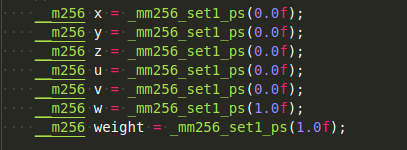
\includegraphics[width=4in]{imagenes/det_vec1.png}
\end{frame}

\begin{frame}
    \frametitle{Detalle de la vectorización}
    
\includegraphics[width=2in]{imagenes/comp_vec2.png} \pause
    
\includegraphics[width=2in]{imagenes/det_vec2.png}
\end{frame}

\begin{frame}
    \frametitle{Detalle de la vectorización}
    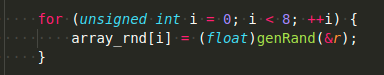
\includegraphics[width=4in]{imagenes/detalle_vec3.png}
\end{frame}

\begin{frame}
    \frametitle{Detalle de la vectorización}
    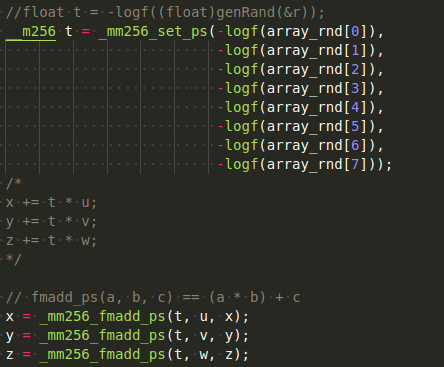
\includegraphics[width=4in]{imagenes/detalle_vec4.png}
\end{frame}

\begin{frame}
    \frametitle{Detalle de la vectorización}
    tinymc sin vectorizar
    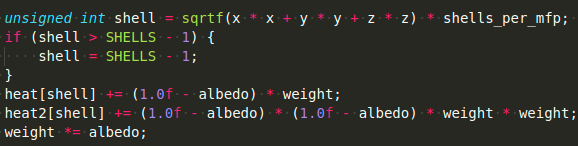
\includegraphics[width=4in]{imagenes/comp_tinymc2.png}
\end{frame}

\begin{frame}
    \frametitle{Detalle de la vectorización}
    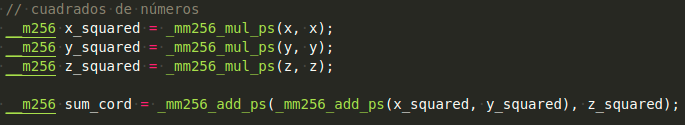
\includegraphics[width=4in]{imagenes/det_vec5.png}
\end{frame}

\begin{frame}
    \frametitle{Detalle de la vectorización}
    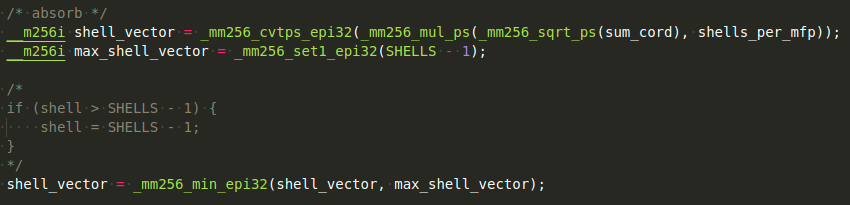
\includegraphics[width=4in]{imagenes/detalle_vec6.png}    
\end{frame}

\begin{frame}
    \frametitle{Detalle de la vectorización}
    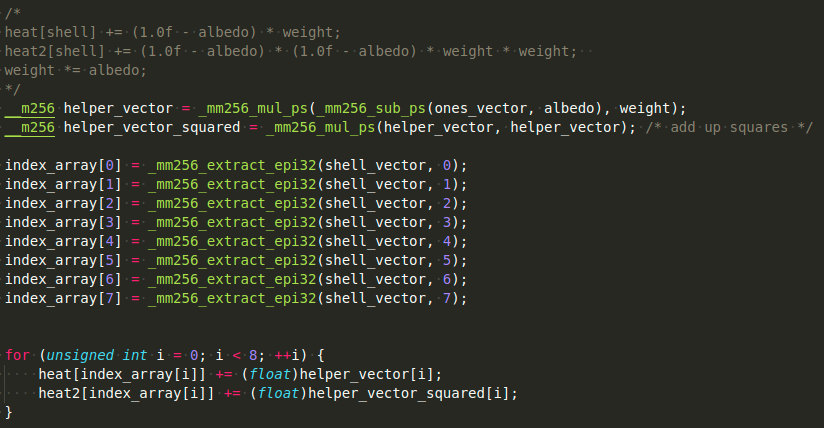
\includegraphics[width=4in]{imagenes/detalle_vec7.png}    
\end{frame}

\begin{frame}
    \frametitle{Detalle de la vectorización}
    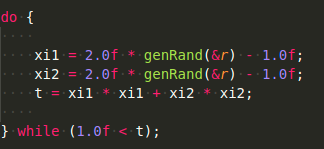
\includegraphics[width=4in]{imagenes/comp_tinymc3.png}
\end{frame}

\begin{frame}
    \frametitle{Detalle de la vectorización}
    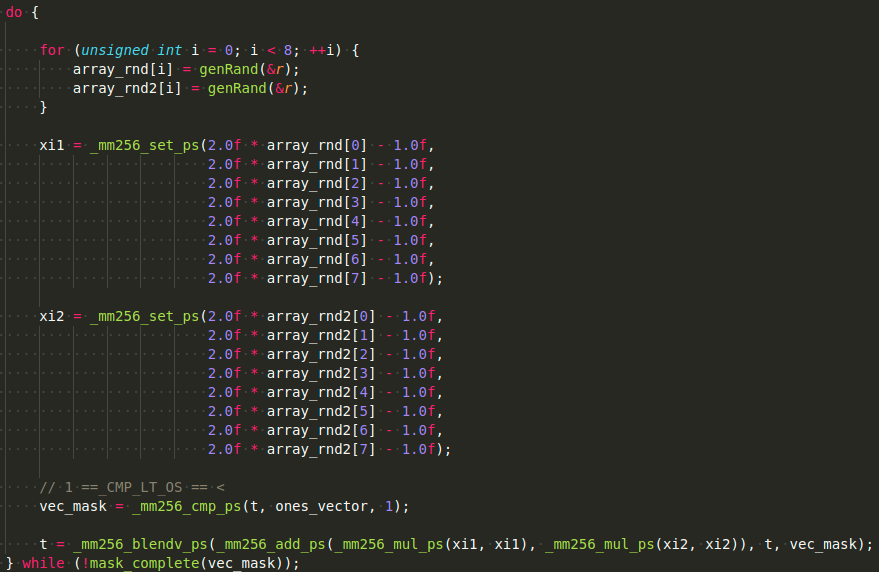
\includegraphics[width=4in]{imagenes/det_vec8.png}
\end{frame}

\begin{frame}
    \frametitle{Detalle de la vectorización}
    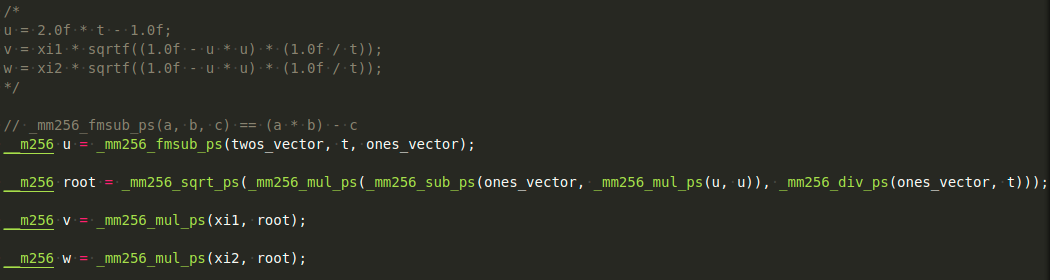
\includegraphics[width=4in]{imagenes/det_vec9.png}
\end{frame}

\begin{frame}
    \frametitle{Detalle de la vectorización}
    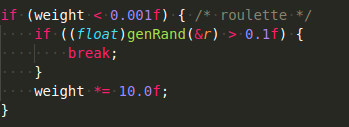
\includegraphics[width=4in]{imagenes/comp_tinymc4.png}
\end{frame}

\begin{frame}
    \frametitle{Detalle de la vectorización}
    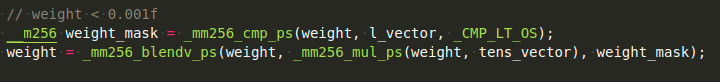
\includegraphics[width=4in]{imagenes/det_vec10.png}
\end{frame}
\begin{frame}
    \frametitle{Detalle de la vectorización}
    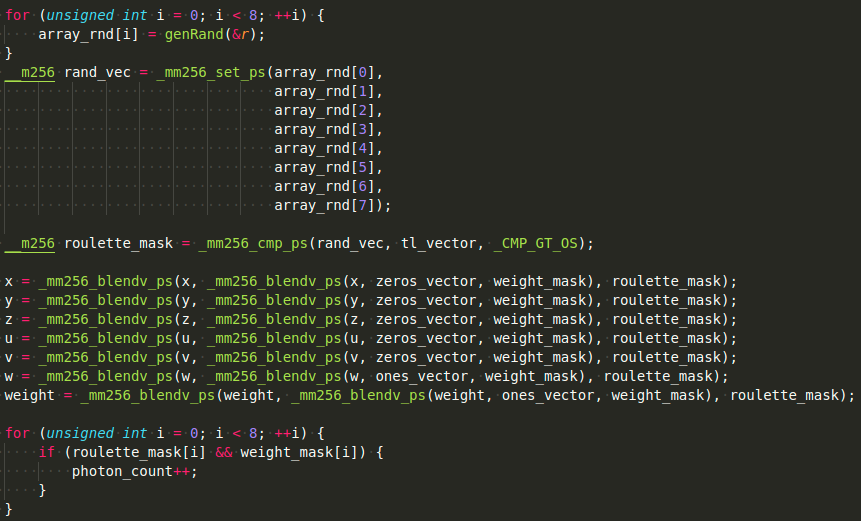
\includegraphics[width=4in]{imagenes/det_vec11.png}
\end{frame}


\end{document}